% =====================================================================
%  Chapter 21 — \idxw{Vantage}: What the Moon Sees That the Earth Does Not
% =====================================================================

\chapter{Vantage: What the Moon Sees That the Earth Does Not}
\label{ch:vantage}

The Moon is not a better telescope than the Earth. It is a different
environment, and three of its environmental differences are quantifiable and
favourable for the specific task this book has in mind. A fourth, which the
concept literature lists as a disadvantage, turns out on inspection to be an
advantage, and that reversal is the pivot on which the whole lunar case
turns.

\section{The sky turns twenty-seven times more slowly}

The Earth rotates once a day, and the sky turns with it at fifteen degrees
an hour. The Moon rotates once every 27.321661 days relative to the stars,
so the lunar sky turns at 13.176 degrees per day. The ratio is
\begin{equation}
\frac{15\ \mathrm{deg\,hr^{-1}}}{13.176\ \mathrm{deg\,day^{-1}}} = 27.4.
\label{eq:skyrate}
\end{equation}

\begin{figure}[!htbp]
\centering
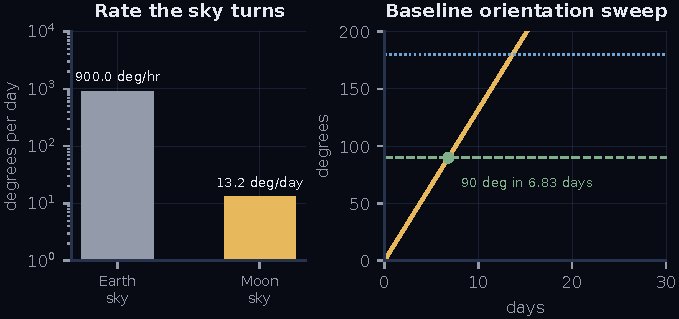
\includegraphics[width=\textwidth]{../figures/fig_rotation.pdf}
\caption{Left: the rate at which the sky turns on the Earth and on the Moon,
on a logarithmic scale. Right: the sweep of a fixed lunar baseline's
orientation, which reaches ninety degrees in under seven days.}
\label{fig:rotation}
\end{figure}

Three consequences follow, and they are of very different kinds.

The first is the observing window. A fixed station on the Earth sees a
target for as long as the target is above the horizon, which at a good
latitude and a good site is a few hours of usable time per night. A fixed
station on the Moon sees a target for as long as the target is above the
lunar horizon, and the lunar sky's slow rotation means that the target's
diurnal motion across the lunar sky is dominated by the target's own proper
motion rather than by the sky's rotation. The access windows are measured in
days rather than hours.

The second is the absence of tracking. Because the sky's rotation is slow,
the pointing is nearly fixed over a campaign, and the integration time is
limited by the target's own motion rather than by a mount. For an
interferometer, whose fringe acquisition needs a stable path difference over
the integration, this matters.

The third is the one the concept literature gets backwards.

\begin{deeper}{The rotation rate as a constraint and as an asset}
The 2003 concept study lists, among the disadvantages of a surface-fixed
interferometer, the fact that ``observations are constrained by the Moon's
rotation rate''. That is true and it is an advantage, because the same
document also states that ``having the interferometer fixed to the lunar
surface keeps the baseline very stable, reducing measurement uncertainties'',
and that ``two measurements at different baseline orientations
(\(\sim\)orthogonal) are required to derive the target's two-angle
position''.

Those two statements are in tension, and the resolution is arithmetic. A
fixed baseline on the Moon sweeps through ninety degrees of orientation in
\(90/13.176 = 6.83\) days. The orthogonal second orientation that the
concept study requires is therefore delivered automatically, within a week,
by the rotation itself, with no moving hardware and no propellant. On the
Earth, the same requirement would need a second instrument or a transport
delay.
\end{deeper}

\section{The Sun-ward blind zone}

The second advantage is geometrical and it is the discovery-side case.

A ground telescope cannot observe close to the Sun: atmospheric scattering
raises the sky background, and the solar avoidance constraints tighten. The
result is the blind zone that the 2026 study of near-Earth-object telescopes
for extreme environments calls the most critical limitation of ground-based
observatories, and it names the historical failures it has caused: 2008~TC3
and 2019~OK, and ``multiple other NEAs detected only days before their
closest approach to Earth''.

The lunar geometry relaxes the constraint. From a polar site\idx{Polar site}, where the Sun
stays low and the sky background is correspondingly low, an observer can see
close to the Sun. The same study publishes the resulting gain as a table of
first detectable distances and extra lead times.

\begin{figure}[!htbp]
\centering
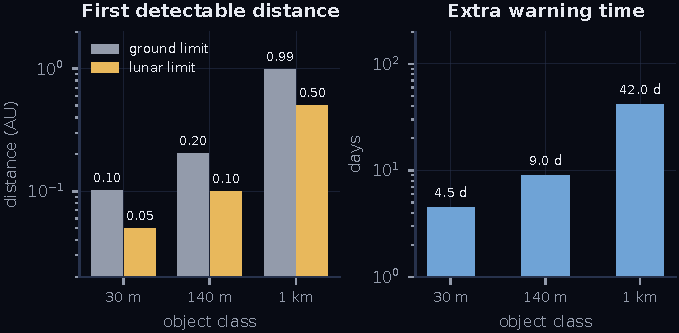
\includegraphics[width=\textwidth]{../figures/fig_sunward.pdf}
\caption{The Sun-ward gain, reconstructed from the published table. Left:
the first detectable distance from the ground and from a lunar observatory.
Right: the extra warning time, at a relative velocity of 20 kilometres per
second.}
\label{fig:sunward}
\end{figure}

\figref{fig:sunward} is worth reading carefully, because it is modest and
the book does not inflate it. A 30-metre object becomes detectable 0.05
astronomical units from the Sun and four to five days earlier. A
140-metre object becomes detectable at 0.10 astronomical units and about nine
days earlier. A one-kilometre object becomes detectable at 0.50 astronomical
units and about six weeks earlier.

Working backwards from the lead times, the ground limits the table implies
are about 0.10 astronomical units for the 30-metre class, 0.20 for the
140-metre class and 0.99 for the kilometre class.

Nine days is not a transformation of planetary defence. What it is, is the
only entry in the table that applies to objects the ground structurally
cannot reach, and it is the entry that matters for the population of Chapter
4: the objects that are still arriving at three thousand a year are the
small, near-Sun ones, and they are the ones the ground finds last.

\section{No atmosphere, and what that is worth}

The third advantage is the one the concept literature lists first, and it is
the least important for this book's proposal, for a reason worth stating.

With no atmosphere there is no scattered light and no airglow, so the diffuse
background at a dark polar site is the zodiacal light and the starlight
alone. The consequence can be computed from the target's own photometry. A
60-metre object at 0.2 astronomical units has an apparent magnitude of 17.2,
and once resolved, a surface brightness of 0.06 magnitudes per square
arcsecond --- about 22 magnitudes above the zodiacal background. At 1.0
astronomical unit its surface brightness is 3.55 magnitudes per square
arcsecond, still about 18 magnitudes above it.

The background is therefore not the constraint on a lunar optical
interferometer. The baseline is. This is worth saying because the intuitive
argument --- ``no atmosphere, so no seeing, so better images'' --- is true
and largely irrelevant to a sixty-metre object seen from a hundred million
kilometres.

\begin{table}[!htbp]
\centering
\small
\caption{The three lunar advantages, and what each one is actually worth
for this task.}
\label{tab:advantages}
\begin{tabularx}{\textwidth}{@{}P{1.33in}P{1.23in}Y@{}}
\toprule
\rowcolor{panel}
\textbf{Advantage} & \textbf{Worth} & \textbf{Comment} \\
\midrule
Slow sky rotation & high & day-long windows, no tracking, and the
orthogonal baseline orientation delivered within 6.83 days \\
\rowcolor{panel}
Sun-ward access & moderate & four to five days for a 30-metre object, nine
days for a 140-metre one \\
No atmosphere & low & the target is 18 to 22 magnitudes above the
background; the baseline is the constraint \\
\bottomrule
\end{tabularx}
\end{table}

\begin{keytakeaways}
\item The lunar sky turns twenty-seven times more slowly than the Earth's,
which gives day-long observing windows and no tracking requirement.
\item The same rotation delivers the orthogonal baseline orientation the
concept study requires within 6.83 days, with no moving hardware.
\item The Sun-ward gain is modest in absolute terms but reaches the only
population the ground structurally cannot see.
\item The absence of atmosphere is the least important of the three: the
target is 18 to 22 magnitudes above the zodiacal background.
\end{keytakeaways}
